\documentclass{article}
\usepackage[utf8]{inputenc} % Required for inputting international characters
\usepackage[T1]{fontenc} % Output font encoding for international characters
\usepackage{amsthm}
\usepackage{wrapfig}
\usepackage{mathpazo} % Use the Palatino font
\usepackage[a4paper, total={5in, 10in}]{geometry}
\usepackage{graphicx} % Required for including images

\usepackage{booktabs} % Required for better horizontal rules in tables

\usepackage{listings} % Required for insertion of code

\usepackage{enumerate} % To modify the enumerate environment
\title{\textbf{Rotacion de un vector \begin{math}\theta \end{math} grados en sentido antihorario.}}
\author{José Juan Suárez Elizalde}
\date{Junio 2020}

\begin{document}

\maketitle
{\fontfamily{qcr}\selectfont
ABSTRACT. 
}
Probaremos que: \begin{math} f(\overrightarrow{v},\theta)=(x\cos\theta -y\sin\theta,y\cos\theta+x\sin\theta)\end{math},
    donde \begin{math} \overrightarrow{v}\end{math} es un vector arbitrario tal que \begin{math}\overrightarrow{v}\in \mathbb{R}2 \end{math} y  \begin{math}\theta\end{math} es los grados que se desea rotar a \begin{math}\overrightarrow{v}\end{math} de su dirección inicial de \begin{math}\lambda\end{math} grados en sentido contrario a las manecillas del reloj. La función nos da el vector resultante en coordenadas rectangulares.
    \\\\
Analicemos:

\begin{wrapfigure}{L}{0.4\textwidth}
  \centering
  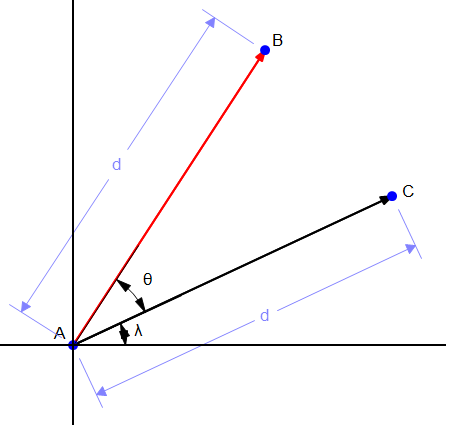
\includegraphics[width=0.4\columnwidth]{1.png}
    Fig. 1 
\end{wrapfigure}
\hfill
\\
\hfill
Tomemos al vector \begin{math}\overrightarrow{v}\end{math} como el vector \begin{math}\overrightarrow{AC}\end{math} representado en \textit{Fig. 1}, el vector resultante (el cual a partir de ahora llamaremos \begin{math}\overrightarrow{r}\end{math} y es representado en Fig. 1 como \begin{math}\overrightarrow{AB}\end{math} tiene que cumplir que \begin{math} \left \| \overrightarrow{r} \right \| = \left \| \overrightarrow{v} \right \| \end{math}, puesto que lo unico que queremos hacer es cambiar su dirección, no su norma.\\
Si tenemos que \begin{math}\overrightarrow{v}\end{math} tiene un angulo \begin{math}\lambda\end{math} con respecto al eje de las abscisas y queremos añadir \begin{math}\theta\end{math} grados a este, entonces si el angulo de \begin{math}\overrightarrow{r}\end{math} es \begin{math}\omega\end{math}, tenemos que: 
\begin{equation}\omega=\lambda+\theta\end{equation}

\begin{wrapfigure}{r}{0.4\textwidth}
  \centering
  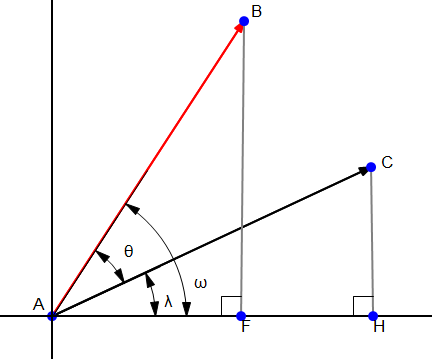
\includegraphics[width=0.4\columnwidth]{2.png}
    Fig. 2
\end{wrapfigure}
\hfill
\\
\hfill
Podemos observar que al cambiar el angulo de nuestro vector, algo mas cambia, ya vimos que la magnitud del vector no, pero si tomamos el sistema de coordenadas que representa a nuestro vector como el sistema rectangular, entonces podemos ver dos parametros representandolo, estos a su vez pueden ser vistos como catetos y la magnitud de nuestro vector seria la hipotenusa, de esta forma transformamos nuestro vector a un triangulo rectangulo.\\
Con esta perspectiva nos damos cuenta que queremos transformar un triangulo rectangulo en otro, pero con el angulo entre el cateto adyacente y la hipotenusa modificado con las restricciones ya anteriormente mencionadas, ademas tambien podemos observar que si encontramos el tamaño de los catetos del triangulo resultante, podremos expresar el vector resultante y el problema estaría resuelto.\\
En Fig. 2 tenemos que los catetos del vector original  \begin{math}\overrightarrow{v}\end{math}, son 
\begin{math}\overrightarrow{HC}\end{math} que representaria a \textit{y} y \begin{math}\overrightarrow{AH}\end{math} que representaria a \textit{x}, tal que \begin{math}
\overrightarrow{v} = (x,y)\end{math}, queremos encontrar \begin{math}\overrightarrow{r}\end{math} que es igual a \begin{math}(x',y')\end{math}, punto que no conocemos.\\
Usemos identidades trigonometricas conocidas para despejar el valor de \textit{x'} y \textit{y'}.
\begin{equation}
    \sin(\omega)=\frac{y'}{ \left \| \overrightarrow{r} \right \|}
\end{equation}
Por \textit{(1)} tenemos que \textit{(2)} es:
\begin{equation}
    \sin(\lambda + \theta)=\frac{y'}{ \left \| \overrightarrow{r} \right \|}
\end{equation}
Con base al mismo razonamiento tenemos que :
\begin{equation}
    \cos(\lambda + \theta)=\frac{x'}{ \left \| \overrightarrow{r} \right \|}
\end{equation}
Podemos usar las siguientes entidades trigonometricas:
\setcounter{equation}{0}
\begin{equation}
    \sin(\lambda + \theta)= \sin{\lambda}\cos{\theta}+\cos{\lambda}\sin{\theta}
\end{equation}
\begin{equation}
    \cos(\lambda + \theta)= \cos{\lambda}\cos{\theta}+\sin{\lambda}\sin{\theta}
\end{equation}
Sustituyendo las identidades en \textit{(3)} y \textit{(4)} tenemos:
\setcounter{equation}{4}
\begin{equation}
   \frac{y'}{ \left \| \overrightarrow{r} \right \|} =  \sin{\lambda}\cos{\theta}+\cos{\lambda}\sin{\theta}
\end{equation}
\begin{equation}
   \frac{x'}{ \left \| \overrightarrow{r} \right \|} =  \cos{\lambda}\cos{\theta}+\sin{\lambda}\sin{\theta}
\end{equation}
Pasa que al tener \textit{(x,y)}, podemos encontrar el valor numerico de las funciones trigonometricas en función de \begin{math}\lambda\end{math}. Las funciones que podemos sustituir en \textit{(5)} y \textit{(6)}, serian \textit{(cos)} y \textit{(sen)}. Encontremoslas: 

\begin{equation}
   \cos(\lambda) = \frac{x}{\left \| \overrightarrow{v} \right \|}
\end{equation}
\begin{equation}
   \sin(\lambda) = \frac{y}{\left \| \overrightarrow{v}\right \|}
\end{equation}
Sustituyamos \textit{(7)} y \textit{(8)} en \textit{(5)} y \textit{(6)}.
\begin{equation}
   \frac{y'}{ \left \| \overrightarrow{r} \right \|} =  \frac{y}{\left \| \overrightarrow{v}\right \|}\cos{\theta}+\frac{x}{\left \| \overrightarrow{v} \right \|}\sin{\theta}
\end{equation}
\begin{equation}
   \frac{x'}{ \left \| \overrightarrow{r} \right \|} =  \frac{x}{\left \| \overrightarrow{v} \right \|}\cos{\theta}+\frac{y}{\left \| \overrightarrow{v}\right \|}\sin{\theta}
\end{equation}
Pasamos \begin{math}
\left \| \overrightarrow{r} \right \|
\end{math} multiplicando en ambas ecuaciones y cancelamos los \begin{math}
\left \| \overrightarrow{v} \right \|
\end{math}, puesto que \begin{math} \left \| \overrightarrow{r} \right \| = \left \| \overrightarrow{v} \right \| \end{math}. Por tanto:
 \begin{equation}
   y'=  y\cos{\theta}+x\sin{\theta}
\end{equation}
\begin{equation}
   x'=  x\cos{\theta}+y\sin{\theta}
\end{equation}
Sí \begin{math}
\overrightarrow{r} = (x',y')
\end{math} entonces sustituimos \textit{(11)} y \textit{(12)}, por lo que tenemos:
 \begin{equation}
   \overrightarrow{r}=( x\cos{\theta}+y\sin{\theta},y\cos{\theta}+x\sin{\theta})
\end{equation}
\qed
\end{document}